\documentclass[10pt,a4paper]{article}
\usepackage[utf8]{inputenc}
\usepackage[german]{babel}
\usepackage{mathrsfs}
\usepackage{amsmath}
\usepackage{amsfonts}
\usepackage{amssymb}
\usepackage{amsthm}
\usepackage[left=2cm,right=2cm,top=2cm,bottom=2cm]{geometry}
\usepackage{minted}
\usepackage{graphicx}

\begin{document}

\section{Number of dice thrown}

For $n$ dice, it is fairly easy, so compute the probability for each possible
outcome. Now it would be interesting to do the opposite. So for a given
outcome/sum of sides $D$ we would like to have a distribution over the number of
dice $n$.

\subsection{Approximation with probabilistic programming}

Probabilistic programming can give us an approximation of the distribution
easily. You just have to program, how you pick an $n$ and sample a $D$ for
it. To reverse the process, you sample from this program a lot of times and
everytime the sampled $D$ equals your expected $D$ you report the $n$ you
picked. Then the histogram over the reported $n$ approximates the true
distribution of $p(n | D)$.

\begin{figure}[h]
  \centering
  \begin{minted}{scheme}
    (define dice-sides (range 1 6))

    (define (number-rolls N)
      (let ((dice (range 1 N)))
        (rejection-query
         (define n (uniform-draw dice))
         (define sum-faces (sum (repeat n (lambda () (uniform-draw dice-sides)))))
         n
         (condition (= sum-faces N)))))

    (hist (repeat 100000 (lambda () (number-rolls 20))))
  \end{minted}
  \caption{A probabilistic progam written in church}
\end{figure}
\begin{figure}[h]
  \centering
  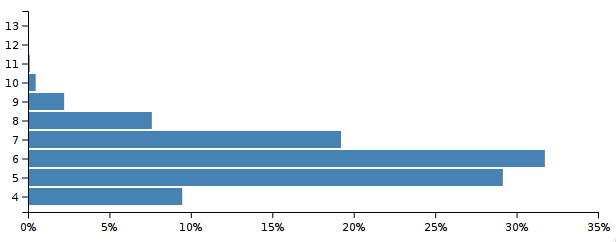
\includegraphics[width=350pt]{church-approx}
  \caption{Approximate distribution of $p(n | D = 20)$ with $100\,000$ iterations}
\end{figure}

\subsection{Analytic examination}

Let $s$ be the number of sides of the dice, $n$ the number of dice and $D$ the
desired result. We start with a uniform prior $n$.
\begin{equation}
  p(n) = \mathbb{U}\left( \lceil \frac{D}{s} \rceil, \dots, D \right)
\end{equation}
The maximum considered number of dice is $D$, because the minimum sum of sides
for $D + 1$ dice is $D + 1$.

WolframAlpha says, that the probabilty of obtaining $D$ on $n$ $s$-sided dice is
\begin{equation}
  P(D | n) = \frac{1}{s^{n}} \sum_{k = 0}^{\lfloor (p - n) / s \rfloor} (-1)^{k} \binom{n}{k} \binom{p - sk - 1}{n - 1}
\end{equation}

The marginal probability of $D$ can be computed with marginalization
\begin{align*}
  P(D) & = \sum_{n = \lceil \frac{D}{s} \rceil}^{D} p(n) \cdot p(D | n)\\
       & = \sum_{n = \lceil \frac{D}{s} \rceil}^{D} \frac{1}{1 + D - \lceil \frac{D}{s} \rceil} \frac{1}{s^{n}} \sum_{k = 0}^{\lfloor (p - n) / s \rfloor} (-1)^{k} \binom{n}{k} \binom{p - sk - 1}{n - 1}\\
       & = \frac{1}{1 + D - \lceil \frac{D}{s} \rceil} \sum_{n = \lceil \frac{D}{s} \rceil}^{D} \frac{1}{s^{n}} \sum_{k = 0}^{\lfloor (p - n) / s \rfloor} (-1)^{k} \binom{n}{k} \binom{p - sk - 1}{n - 1}\\
\end{align*}
For me that is as closed form, as it gets. Plugging it into the below formula,
will give us the posterior.
\begin{equation}
  p(n | D) = \frac{p(D | n) \cdot p(n)}{p(D)} = \frac{\frac{1}{s^{n}} \sum_{k = 0}^{\lfloor (p - n) / s \rfloor} (-1)^{k} \binom{n}{k} \binom{p - sk - 1}{n - 1}}{\sum_{n = \lceil \frac{D}{s} \rceil}^{D} \frac{1}{s^{n}} \sum_{k = 0}^{\lfloor (p - n) / s \rfloor} (-1)^{k} \binom{n}{k} \binom{p - sk - 1}{n - 1}}
\end{equation}

This can be plotted with the following julia code
\begin{minted}{julia}
using Gadfly

s = 6
D = 20
ns = ceil(D / s):D

toInt(n) = convert(Integer, n)

function pDn(D, n)
    binom(a, b) = binomial(toInt(a), toInt(b))
    term(k) = (-1)^k * binom(n, k)) * binom(D - s * k - 1, n - 1)
    series = [term(k) for k = 0:floor((D - n) / s)]

    (1 / s^n) * sum(series)
end

function pnD(n, D)
    pDn(D, n) / sum([pDn(D, k) for k = ceil(D / s):D])
end

ps = [pnD(n, D) for n in ns]

plot(x=ps, y=ns,
     Geom.bar(orientation=:horizontal),
     Guide.xlabel("Probability p(n | 20)"),
     Guide.ylabel("Number of dice n"),
     Coord.cartesian(ymin=4, ymax=13))
\end{minted}
\begin{figure}[h]
  \centering
  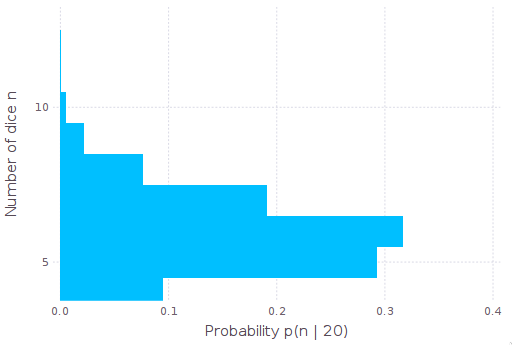
\includegraphics[width=300pt]{julia-exact}
  \caption{Exact distribution}
\end{figure}
The approximate and exact distributions are visually indistinguishable.

\end{document}